\documentclass[tikz,border=2pt]{standalone}
\usetikzlibrary{arrows.meta,patterns}
\begin{document}
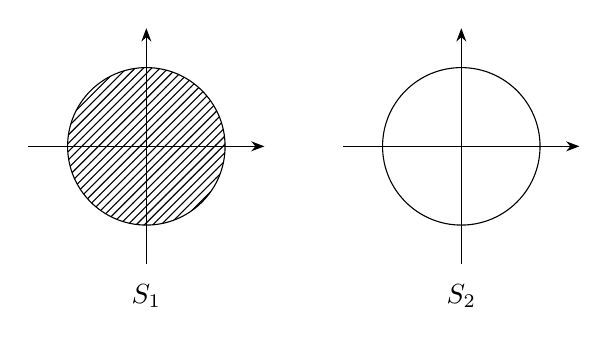
\begin{tikzpicture}[>=Stealth]
    % S_1 : x^2 + y^2 <= 1
    \begin{scope}
        \draw[->] (-1.5,0) -- (1.5,0);
        \draw[->] (0,-1.5) -- (0,1.5);
        \draw[pattern=north east lines] (0,0) circle (1);
        \node at (0,-1.9) {$S_1$};
    \end{scope}
    % S_2 : x^2 + y^2 = 1
    \begin{scope}[xshift=4cm]
        \draw[->] (-1.5,0) -- (1.5,0);
        \draw[->] (0,-1.5) -- (0,1.5);
        \draw (0,0) circle (1);
        \node at (0,-1.9) {$S_2$};
    \end{scope}
\end{tikzpicture}
\end{document}
